% SSAC27 research paper, draft 2. Structure follows paper/paper-outline.md (v4).
% Abstract is Nate's paper/abstract.tex verbatim (number fixes only: 6.5 million, 113 to 451, 6 heads).
% Compile with pdfLaTeX from paper/draft2. Every number is from the clean build (career
% pitcher-batters excluded). Sources are cited in comments beside each number.

\documentclass[11pt,letterpaper]{article}
% Layout follows the SSAC "Paper Template": 1in sides, 1.1in top, 1.2in bottom,
% Cambria 11pt single spaced with 11pt after each paragraph, 42 Analytics logo bottom left.
\usepackage[left=1in,right=1in,top=1.1in,bottom=1.2in,footskip=0.3in]{geometry}
\usepackage[T1]{fontenc}
\usepackage{caladea}      % metric-compatible free clone of Cambria
\usepackage{amsmath}
\usepackage{amssymb}
\usepackage{booktabs}
\usepackage{graphicx}
\graphicspath{{figs/}{./}}
\usepackage{xcolor}
\usepackage{tikz}
\usetikzlibrary{arrows.meta,positioning,fit,calc,shapes.geometric,backgrounds}
\newcommand{\toreview}{\textcolor{red}{\textbf{[TO REVIEW]}}~}
\usepackage[numbers]{natbib}
\setlength{\bibsep}{3pt}
\usepackage{titlesec}
\usepackage{fancyhdr}
\usepackage{eso-pic}
\usepackage{hyperref}
\hypersetup{colorlinks=true,linkcolor=black,citecolor=black,urlcolor=blue}

\setlength{\parindent}{0pt}
\setlength{\parskip}{11pt}
\titleformat{\section}{\fontsize{16}{19}\selectfont\bfseries}{\thesection.}{0.4em}{}
\titleformat{\subsection}{\fontsize{12}{14}\selectfont\bfseries}{\thesubsection.}{0.4em}{}
\titleformat{\paragraph}[runin]{\normalsize\bfseries}{}{0pt}{}
\titlespacing*{\section}{0pt}{6pt}{0pt}
\titlespacing*{\subsection}{0pt}{0pt}{-8pt}
\titlespacing*{\paragraph}{0pt}{0pt}{0.6em}

\pagestyle{fancy}
\fancyhf{}
\renewcommand{\headrulewidth}{0pt}
\cfoot{\thepage}
\AddToShipoutPictureBG{\AtPageLowerLeft{\hspace*{0.9in}\raisebox{0.38in}{
\includegraphics[width=1.95in]{42analytics-logo.png}}}}

\newcommand{\papertitle}{Conditional Queries Against a Learned Hitter Process Model}
\newcommand{\papertrack}{Baseball}  % TODO: confirm track
\newcommand{\paperid}{Paper ID}     % TODO: SSAC paper ID

\begin{document}
\raggedright
\thispagestyle{fancy}
\begin{center}
{\fontsize{18}{22}\selectfont\bfseries \papertitle\par}
\vspace{11pt}
{\fontsize{14}{17}\selectfont \papertrack\par \paperid\par}
\end{center}

% Nate's abstract (paper/abstract.tex), verbatim except 5 heads -> 6 (approved 2026-10-31).
% Its Table 1 is in Section 3.1 and its Figure 1 is the Introduction teaser.
\section*{Abstract}
In baseball, understanding how to use great hitters is often a simple task: play as many of them as you can and play them often. Teams try to gain an edge with the remaining hitters, but less playing time means thinner data in an area that takes hundreds of plate appearances to stabilize. This paper asks whether a model trained on pitches can project how a hitter will do against a type of matchup, like handedness or a specific pitcher, with less data than standard projections need.

We train a neural network inspired by (batter$|$pitcher)2vec that learns player embeddings from hitter-controlled pitch outcomes, which decreases the impact of outcome luck. A plate appearance is broken into 6 heads: swing decision, contact, and quality decomposed as exit velocity, launch angle, and spray direction, each conditioned on the pitcher and the game state. The model trains on 6.5 million Statcast pitches from 2015 through 2024 covering 1,672 hitters, each represented as a 64-dimensional embedding. To query it, we reweight which pitchers the projection is drawn over and compose the outputs through the count-state Markov chain into a projected wOBA, so a new split needs a new weight vector, not a retrained model. We test side-specific wOBA against left- and right-handed pitchers on sealed 2025 data against gradient-boosted and empirical Bayes baselines, using RMSE and weighted rank correlation, grouped by prior plate appearances (PA, Table~1).

The model did not pass our pre-registered test. Pooled RMSE was tied (0.0452 against 0.0453 for gradient boosting and 0.0460 for empirical Bayes) and pooled rank correlation was higher (0.47 against 0.42 and 0.40). It beat both baselines on both measures only for hitters with 113 to 451 prior plate appearances, an exploratory result. On 2024, the season used to select the model, it recovers 60\% of the rank-order signal and 64\% of the level signal that one season of data can measure. Without being given definitions of power or contact, the embedding still separates hitters on both, with held-out accuracy of 0.79 and 0.75 against 0.33 by chance, and observed wOBA rises toward high power and high contact (Figure~1).

The model is better at ordering hitters within a split than at predicting how many points of wOBA the split is worth. For a team, that makes it most useful for ranking platoon options among hitters with a moderate track record, where the decision is actually in question, not as a replacement for a projection system on raw accuracy.

% =====================================================================================
\section{Introduction}
\label{sec:intro}

% Source: src/analysis/claim1_eval.py STABILIZATION_N_STAR = 226 (variance-components estimate
% on training seasons, hitters only).
Most of a lineup decides itself. A team's best hitters play every day against every kind of pitcher, and nobody needs a model to tell them to. The decisions with room for an edge are about everyone else, the bench bats and platoon hitters, and those decisions usually turn on a split, how a hitter does against one kind of pitcher. The hitters a team is least sure about are also the ones with the least playing time, and a split takes a long time to settle. On our training seasons, a hitter's wOBA against left-handed pitchers, the level and not yet the gap between his two sides, needs about 226 plate appearances (PA) against them before half of its variance across hitters is signal rather than noise. A part-time hitter can take seasons to get there, and the decision has to be made long before then.

Part of why a split settles so slowly is that wOBA is measured at the end of a plate appearance, and a lot of what decides it is out of the hitter's hands. The fielders, the park, and where a ball in play happens to land all move the result. What the hitter does control happens earlier and more often. On every pitch he decides whether to swing, and when he swings he either makes contact or misses. When he puts the ball in play, Statcast records how hard he hit it, at what launch angle, and in which direction. A plate appearance produces one wOBA value but several of these pitch-level outcomes, and they carry less of the luck that a result picks up after the ball leaves the bat.

% Source: ~/os/knowledge/library/baseball-research/alcorn-2018-batter-pitcher2vec.pdf, Sections 2.1,
% 2.2 and 4 (Retrosheet 2013 to 2015 at-bats, nine-dimension embeddings, softmax over at-bat outcomes,
% PITCHf/x suggestion in Future directions).
\citet{alcorn2018} showed that a network can learn useful descriptions of players from their matchups alone. The (batter$|$pitcher)2vec model gave every batter and pitcher a nine-dimension embedding and trained it to predict the outcome of each at-bat from the identities of the two players, using Retrosheet data from 2013 through 2015. The embeddings grouped similar hitters together without being told what made them similar, and they predicted outcome distributions for matchups that never occurred in training slightly better than simpler approaches. In the paper's future directions, Alcorn suggested that working with PITCHf/x measurements instead of discrete outcomes could carry more information about a player's physical characteristics. We take a related step with Statcast. The pitch's tracking measurements become the input, and the hitter's tracked response to the pitch becomes the target. Our network keeps the idea of a learned embedding for each hitter, but it predicts what the hitter does with each pitch rather than how the at-bat ends, and it is conditioned on the pitch itself rather than on the pitcher's identity.

% Source: ~/os/knowledge/library/baseball-research/tango-2009-the-book-p157-platoon-constants.md
% (The Book p.157: RHB 2,200 PA vs LHP to reach half weight, LHB about 1,000).
The standard way to estimate a platoon split is to regress the hitter's observed split toward the league split for his side. In \citet[p.~157]{tango2007}, a right-handed hitter needs about 2,200 PA against left-handed pitchers before his own split gets half the weight, and a left-handed hitter about 1,000. Very few hitters ever face that many left-handers, so for most of them the estimate stays close to the league average. Our empirical Bayes baseline is the same kind of shrinkage \citep{efron1972}, with the correlation between a hitter's two sides estimated from the data rather than fixed. It is one of the two bars a new method has to clear, and the other is a gradient-boosted model given the same pitch-level information ours sees.

This paper asks whether a model trained on pitches can project how a hitter will do against a type of matchup with less data than standard projections need. We make three contributions. The first is the model and a way to query it. A query picks the pitchers a projection is drawn over, and the model's per-pitch outputs are composed through the count into a projected wOBA, so a new split needs a new set of pitcher weights and not a new model. The second is a pre-registered test of the handedness query on sealed 2025 data against gradient-boosted and empirical Bayes baselines. The model did not pass it. In the low-exposure stratum the test was decided on, it beat neither baseline. Across all hitters its error tied the baselines and it ordered hitters better than both, and it beat both on both measures among hitters with 113 to 451 prior PA against that hand, which we report as exploratory. The third is a look inside the embedding. Trained only on per-pitch outcomes, with no hitter-level statistics, it separates hitters by power and by contact rate (Figure~\ref{fig:powercontact}), and it holds a weak but measurable platoon direction. We read these results as a model that orders hitters better than it sizes their splits, a reading built mostly on descriptive and exploratory results rather than on the test we registered.

% Source: fig1_power_contact.png (Nate's abstract Figure 1); Section 3.3 numbers.
\begin{figure}[t]
\centering
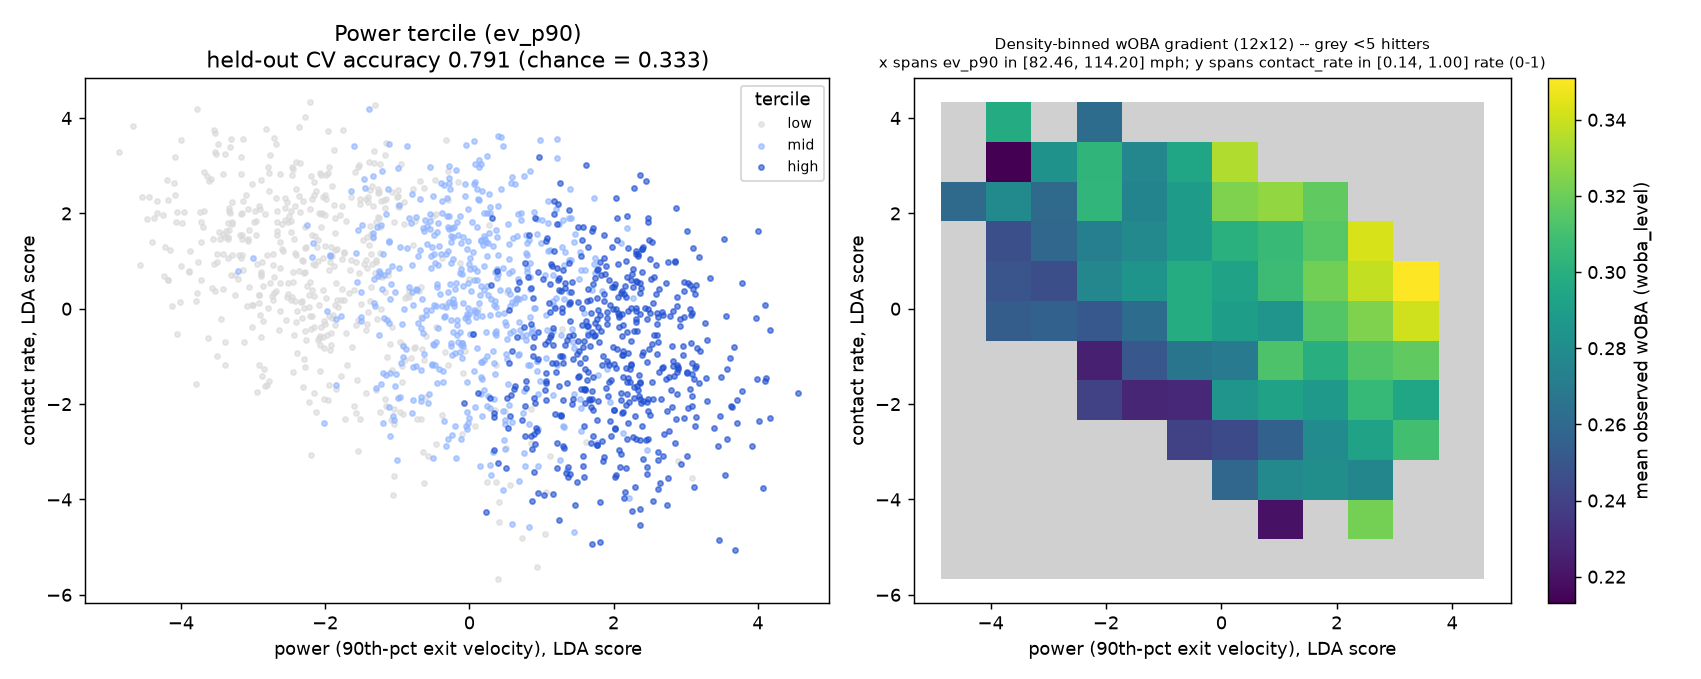
\includegraphics[width=\linewidth]{fig1_power_contact.png}
\caption{\toreview Hitters placed by the embedding on fitted power and contact directions. The left panel colors hitters by observed power tercile, and the right panel shows mean observed wOBA per cell, which rises toward high power and high contact. The model was never told what power or contact is (Section~\ref{sec:embedding}).}
\label{fig:powercontact}
\end{figure}

Section~\ref{sec:methods} describes the data, the model, how a query works, and how we evaluate it. Section~\ref{sec:results} reports the 2025 test, a grade of each hitter's 2025 split, how much of the signal one season of data allows any method to recover, and what the embedding learned. Section~\ref{sec:discussion} makes the case that the model orders better than it sizes, checks that reading against five hitters chosen in advance and against the hitters on whom the model and empirical Bayes disagree most, and lists the limits. Section~\ref{sec:conclusion} lists what we would test next.

% =====================================================================================
\section{Methods}
\label{sec:methods}

We build the model in two parts. A network learns, for each hitter and each pitch, the probability of every outcome the hitter controls. A query then turns those per-pitch probabilities into the number a team would use, a projected wOBA against a chosen set of pitchers. Section~\ref{sec:data} describes the data, Section~\ref{sec:model} the network, Section~\ref{sec:query} the query, and Section~\ref{sec:eval} how we evaluate it.

\subsection{Data}
\label{sec:data}

% Source: data/processed/phase_d5_clean_final/manifest.json; src/data cleaning rules;
% decision log 2026-09-20 (clean build, pitcher-batter rule).
We use pitch-level Statcast data from the 2015 through 2025 regular seasons. Each pitch carries its velocity, movement, release point, spin, location at the plate, pitch type, the count, and the handedness of both players. A ball in play also carries its exit velocity, launch angle, and the coordinates where it was fielded, from which we compute a spray angle. We drop pitchouts, automatic balls and strikes, bunts, pitches thrown by position players, and pitches missing a core measurement. We also remove pitchers who come to the plate, keeping two-way players such as Shohei Ohtani in the hitter pool. After cleaning, the table holds 7,245,923 pitches. The 6,540,616 pitches from 2015 through 2024 train the final model and cover 1,672 hitters and 2,182 pitchers.

% Source: src/config/split_config.json, split_config_final_run.json; decision log 2026-08-01, 2026-09-20.
Every split is by season, fixed before any model was trained. Each modeling choice was made by training on 2015 through 2023 and scoring on 2024, so 2024 is the selection season. The chosen configuration was then retrained from scratch on 2015 through 2024 and scored on 2025, which no model trained on. Inputs that need fitting, such as the scaling of continuous features, are fit on 2015 through 2023 only, and the baselines see only seasons before the one being scored.

\subsection{Model}
\label{sec:model}

% Source: src/model/v1.py (head_swing, head_contact, head_split, head_ev, head_la, head_spray);
% data manifest n_quality_bins 24; decision log 2026-08-08 (three-class contact split, take surface).
Figure~\ref{fig:arch}a shows the network. Each hitter has a 64-dimension embedding, a learned row of numbers that is the only thing the model knows about him. Each pitch is described by a 46-dimension context vector built from the pitch's physical measurements, its location, its type, the handedness of both players, and the count. The pitcher enters only through the pitches he throws, not through an identifier, so the model can describe a pitcher it has seen throw but never faced with this hitter. The count is the only game state the model sees. We left out the score, the inning, and the runners to keep the model about the hitter rather than the situation.

The network passes the context through two layers and joins the result with the hitter's embedding in a shared trunk of two more layers. Six heads read the trunk, in the order a plate appearance unfolds. The swing head gives the probability that the hitter swings, and the contact head the probability that a swing makes contact. A third head splits contact into a foul, a foul tip, or a ball in play, since with two strikes a foul tip is a strikeout and a foul is not. The last three heads describe a ball in play by its exit velocity, launch angle, and spray direction, each cut into 24 bins. Launch angle is predicted given exit velocity, and spray given both, so the model never assumes the three are independent. These are the parts of a plate appearance the hitter controls most directly. What happens on a pitch he takes is mostly up to the pitcher and the umpire, so we read it from a table rather than from the network. The table gives the chance of a ball, a called strike, or a hit batter by plate location, separately for each pairing of batter and pitcher hand, fit on the training seasons.

\begin{figure}[t]
\centering
% fig_arch.tex -- architecture (a) and query (b) schematic. \input inside a figure env.
% needs: tikz with arrows.meta, positioning, fit, calc, shapes.geometric, backgrounds; amsmath; xcolor
\begin{tikzpicture}[
  x=1cm, y=1cm, font=\scriptsize, text=black!80, line width=0.5pt,
  box/.style={draw=black!55, rounded corners=1.5pt, align=center, inner sep=2pt,
              minimum height=0.5cm},
  acc/.style={draw=blue!60, fill=blue!7},
  bar/.style={draw=black!55, fill=black!5, rounded corners=1.5pt,
              minimum width=0.46cm, minimum height=5.6cm},
  head/.style={box, minimum width=3.2cm, anchor=west},
  arr/.style={-{Stealth[length=3.5pt,width=3pt]}, draw=black!60},
  cond/.style={-{Stealth[length=3pt,width=2.6pt]}, draw=blue!60, densely dashed},
  ttl/.style={anchor=west, font=\footnotesize\bfseries},
  note/.style={text=black!60},
  cnt/.style={draw=black!45, rounded corners=1pt, inner sep=0pt, minimum width=0.42cm,
              minimum height=0.26cm, font=\tiny},
  stepc/.style={circle, draw=blue!60, fill=blue!7, inner sep=0pt, minimum size=0.38cm,
                font=\scriptsize\bfseries},
  para/.style={anchor=north west, align=left, inner sep=0pt},
]

% ---------------------------------------------------------------- (a) the network
\node[ttl] at (0,8.55) {(a) The network};

\node[box, acc, minimum width=2.45cm] (hid) at (1.25,7.55) {Hitter ID $h$};
\node[box, acc, minimum width=2.45cm] (emb) at (1.25,6.65) {Embedding (64)};
\node[box, minimum width=2.45cm, text width=2.3cm] (ctx) at (1.25,4.9)
  {Pitch context (46)\\[1pt]{\tiny\color{black!60}physical measurements,
   location, type, handedness of both players, count}};
\node[box, minimum width=2.45cm] (c1) at (1.25,3.45) {Context layer (128)};
\node[box, minimum width=2.45cm] (c2) at (1.25,2.55) {Context layer (128)};
\draw[arr] (hid) -- (emb);
\draw[arr] (ctx) -- (c1);
\draw[arr] (c1) -- (c2);

\node[bar] (cat) at (3.05,5.0) {};
\node[bar] (t1)  at (3.8,5.0)  {};
\node[bar] (t2)  at (4.55,5.0) {};
\node[rotate=90] at (cat) {Concatenate (64 + 128)};
\node[rotate=90] at (t1)  {Trunk layer (256)};
\node[rotate=90] at (t2)  {Trunk layer (256)};
\draw[arr] (emb.east) -- (cat.west |- emb.east);
\draw[arr] (c2.east)  -- (cat.west |- c2.east);
\draw[arr] (cat) -- (t1);
\draw[arr] (t1) -- (t2);

% six heads, top to bottom in plate-appearance order
\foreach \name/\y/\lbl in {
    sw/7.45/{Swing},
    co/6.47/{Contact $\mid$ swing},
    sp/5.49/{Foul/tip/in play $\mid$ contact},
    ev/4.51/{Exit velocity {\color{black!60}(24 bins)}},
    la/3.53/{Launch angle $\mid$ EV {\color{black!60}(24)}},
    sy/2.55/{Spray $\mid$ EV, LA {\color{black!60}(24)}}} {
  \node[head] (\name) at (5.1,\y) {\lbl};
  \draw[arr] (t2.east |- \name.west) -- (\name.west);
}
% EV and LA bins feed the later heads
\draw[cond] (ev.east) to[out=0, in=0, looseness=1.3] (la.east);
\draw[cond] (ev.east) to[out=0, in=0, looseness=1.1] (sy.east);
\draw[cond] (la.east) to[out=0, in=0, looseness=1.3] (sy.east);

\node[box, dashed, draw=black!50, text width=8.1cm, inner sep=3pt] (take) at (4.25,1.3)
  {Take table, fit separately and not part of the network\\[1pt]
   $p(\text{ball},\ \text{called strike},\ \text{HBP} \mid
     \text{location, batter hand, pitcher hand})$};

% panel divider
\draw[black!20] (8.85,0.8) -- (8.85,8.7);

% ---------------------------------------------------------------- (b) a query
\begin{scope}[xshift=9.15cm]
\node[ttl] at (0,8.55) {(b) A query};

% step 1
\node[stepc] (s1) at (0.2,7.9) {1};
\node[para, text width=6.4cm] at (0.55,8.03)
  {For pitcher $j$ and each count, sample 6 real pitches he threw in that count
   to same-side hitters. Run the network for hitter $h$ and average.\\[3pt]
   {\color{blue!60}$\Rightarrow$} per count $p_B$, $p_S$, $p_F$, $p_H$ and $v(b,s)$,
   the expected wOBA from a ball in play\\(its chance times its average value)};

% step 2, the 12-count chain
\node[stepc] (s2) at (0.2,5.5) {2};
\begin{scope}[shift={(0.95,5.5)}]
  \foreach \b in {0,...,3} \foreach \s in {0,1,2}
    \node[cnt] (n\b\s) at (0.62*\b,-0.48*\s) {\b-\s};
  \foreach \b in {0,1,2} \foreach \s in {0,1,2} {
    \pgfmathtruncatemacro{\nb}{\b+1}
    \draw[arr, draw=black!40] (n\b\s) -- (n\nb\s);}
  \foreach \b in {0,...,3} \foreach \s in {0,1} {
    \pgfmathtruncatemacro{\ns}{\s+1}
    \draw[arr, draw=black!40] (n\b\s) -- (n\b\ns);}
  \node[cnt, acc] at (n00) {0-0};
  \node[note, font=\tiny, anchor=south] at ($(n10.north)!0.5!(n20.north)+(0,0.03)$)
    {balls $\rightarrow$};
  \node[note, font=\tiny, anchor=north] at (n12.south |- 0,-1.15) {strikes $\downarrow$};
\end{scope}
\node[para, text width=3.45cm] at (3.3,5.63)
  {Count-state Markov chain over the 12 counts, solved backward from the end states\\[3pt]
   {\color{blue!60}$\Rightarrow$} $W_{hj} = W(0,0)$};

% step 3
\node[stepc] (s3) at (0.2,3.45) {3};
\node[para, text width=6.4cm] at (0.55,3.58)
  {Weighted mean over the pitcher set $S$, with weights proportional to batters faced};
\node[anchor=west] at (0.5,2.42)
  {$\widehat{\text{wOBA}}_S(h)=\sum_j w^S_j\, W_{hj}, \qquad
    w^S_j\propto \text{BF}_j\,\mathbf{1}[j\in S]$};
\node[box, draw=blue!60, text width=6.2cm, inner sep=3pt, anchor=north west]
  at (0.55,1.98) {A new split is a new set $S$, so only the weights change.
                 No retraining.};

\draw[arr] (s1) -- (s2);
\draw[arr] (s2) -- (s3);
\end{scope}
\end{tikzpicture}

\caption{\toreview (a) The network. A hitter's embedding and the pitch context feed a shared trunk, and six heads predict the hitter-controlled outcomes of the pitch in the order they happen. Taken pitches are read from a separate table. (b) A query. Per-count pitch outcomes for one pitcher are composed through the count into $W_{hj}$, and a weighted average over the chosen pitchers gives the projection. A new split changes only the weights.}
\label{fig:arch}
\end{figure}

% Source: src/model/v1.py loss; src/model/train.py masks.
The network is trained to maximize the summed log-likelihood of what each hitter did,
\begin{equation}
\mathcal{L} = \sum_{i} \Big[ \log p(a_i) + m^{c}_i \log p(c_i) + m^{t}_i \log p(t_i \mid c_i) + m^{e}_i \log p(e_i) + m^{l}_i \log p(l_i \mid e_i) + m^{s}_i \log p(s_i \mid e_i, l_i) \Big],
\label{eq:loss}
\end{equation}
where for pitch $i$, $a_i$ is the swing decision, $c_i$ the contact outcome, $t_i$ whether contact was a foul, a foul tip, or a ball in play, and $e_i$, $l_i$, and $s_i$ the exit velocity, launch angle, and spray bins. Every probability is also conditioned on the hitter and the pitch context. Each mask $m_i$ is one when that outcome exists and was measured, so contact is scored only on swings, the split only on contact, and the three quality terms only on measured balls in play.

% Source: results/checkpoints/clean_dim64_final_s0.pt (266,317 parameters, batch 8192, lr 1e-3,
% step budget 18,538); results/model_v1/sweep_log.csv stage clean; decision log 2026-09-04.
The whole network has 266,317 parameters. We chose among a small set of configurations, varying the embedding size and how strongly the embeddings are regularized, by log loss on 2024, and the 64-dimension embedding scored best. The final model was retrained on 2015 through 2024 for a fixed number of steps, set by the median best stopping point of the five selection runs, because the refit has no later season to stop on. We train five copies from different random seeds, a deep ensemble \citep{lakshminarayanan2017}, and before any query we average each head's predicted distribution across the five.

\subsection{Querying the model}
\label{sec:query}

% Source: src/model/query.py docstring; src/model/query_tables.py; decision log 2026-08-08 (exact
% solve, pitcher population weighted by batters faced, ensemble averages conditionals).
The network answers a question about one pitch, and a team asks about many plate appearances against many pitchers. A query connects the two in three steps, traced in Figure~\ref{fig:arch}b.

The first step fixes one pitcher. For pitcher $j$ and each count, we draw six real pitches he threw in that count to hitters of the same side during the training seasons, run them through the network for hitter $h$, and average. When a pitcher threw too few pitches in a count, the draw falls back to the same number of strikes and then to all his pitches to that side. That gives, for each count, the probability that the next pitch ends as a ball, a strike, a foul, a hit batter, or a ball in play, and the expected wOBA a ball in play adds, its probability times its average value. That average value sums, over every combination of exit velocity, launch angle, and spray bins, the hitter's predicted chance of the combination times the league's average wOBA for it, and a ball in play without measurements gets the league's average value for those.

The second step plays out the plate appearance. Given the pitch, the count changes like a Markov chain over 12 states, from 0-0 to 3-2, and the expected wOBA from count $(b,s)$ satisfies
\begin{equation}
W(b,s) = p_B\, W(b+1,s) + p_S\, W(b,s+1) + p_F\, W(b,\min(s+1,2)) + p_H\, w_{\text{HBP}} + v(b,s),
\label{eq:chain}
\end{equation}
where $p_B$, $p_S$, $p_F$, and $p_H$ are the chances of a ball, a strike, a foul, and a hit batter in that count, $v(b,s)$ is the expected value from a ball in play, a fourth ball is worth a walk's wOBA weight, and a third strike is worth zero. With two strikes a foul leaves the count where it was, and the equation can be solved for that loop directly. Working backward from the end states gives $W_{hj} = W(0,0)$, the hitter's projected wOBA in one plate appearance against pitcher $j$, without simulating any plate appearances.

The third step chooses the pitchers. A query $S$ is a set of pitchers, and the projection is their weighted average,
\begin{equation}
\widehat{\text{wOBA}}_S(h) = \sum_{j} w^S_j \, W_{hj}, \qquad w^S_j \propto \text{BF}_j \, \mathbf{1}[j \in S],
\label{eq:query}
\end{equation}
where $\text{BF}_j$ is pitcher $j$'s batters faced in the training seasons. For a platoon split, $S$ is every left-handed or every right-handed pitcher. Pitchers who throw hard, pitchers who live at the top of the zone, or one named pitcher are the same calculation with a different $S$, and none of them needs the model to be retrained. In this paper we test only the handedness query. The others run through the same code but have not been checked against outcomes.


\subsection{Evaluation}
\label{sec:eval}

% Source: src/analysis/claim1_eval.py (STABILIZATION_N_STAR = 226, strata at n*/2 and 2n*, eval floor
% 10 PA); results/model_evaluation_final_clean/model_v1_claim1_verdict_min_pa_sweep_clean_dim64_final.json.
We test only the handedness query, and we make the paper's question, whether the model needs less data than standard projections, concrete through prior exposure. We score a hitter's wOBA against one pitcher hand in one season, and we call that a unit. Units are grouped by prior exposure, the hitter's PA against that hand in every season before the one being scored. The cuts are at 113 and 452 PA, half and twice the 226 PA at which side-specific wOBA against left-handers stabilizes in our training data. The low stratum has fewer than 113 prior PA, the medium stratum 113 to 451, and the high stratum 452 or more. A unit needs at least 10 PA in the scored season to count. Raising that floor to 25 or 50 PA removes units but leaves every result in Section~\ref{sec:test} passing or failing the same way. Two more targets come from the same projections. The level is a hitter's wOBA pooled over both hands, and the platoon split is his wOBA against left-handers minus his wOBA against right-handers.

% Source: decision log 2026-07-29 (ladder), 2026-08-08; src/analysis/baseline_ladder_bivariate_eb.py
% docstring (TRAILING_SEASONS = 3, covariance by batter type, 50-PA floor for the cross term).
We compare the model with two baselines. The empirical Bayes baseline takes a hitter's wOBA against each hand over the previous three seasons and shrinks the two sides toward the league average for their batting type (left, right, or switch) together, with the correlation between the sides estimated from the data \citep{efron1972}. It generalizes the platoon regression of \citet{tango2007}, learning the amount of shrinkage from the data rather than fixing it, and it is a standard public method. The boosted baseline is gradient-boosted trees \citep{chen2016} fit on one row per hitter, season, and pitcher hand. It sees the same trailing outcomes plus summaries of the hitter's own pitches, such as swing, whiff, and exit velocity rates, aggregated by pitcher hand and coarse pitch group. It does not see the individual pitches the model reads, the pitchers, or the full count. Neither baseline ever sees the season it is scored on.

% Source: claim1_eval.py docstring; decision log 2026-07-30 (beat both or claim nothing, "in the
% claimed stratum"), 2026-08-01 (weighted rank); paired CSV (2,000 batter-clustered draws).
Two measures score each method, both weighted by each unit's PA in the scored season. Root mean squared error (RMSE) asks how close the projected wOBA is to what happened, and the weighted Spearman rank correlation asks whether the method puts the hitters in the right order. Each comparison between the model and a baseline is a paired difference with a 95\% interval from 2,000 bootstrap draws that resample batters, so a hitter who appears against both hands moves as one. We registered one test before the 2025 model was trained. In the low stratum, where the data are thinnest and the question matters most, the model had to beat the boosted baseline on error and both baselines on order. That is the only confirmatory comparison in the paper. Every other comparison, pooled over strata or within the medium or high stratum, is exploratory.

% Source: src/config/split_config.json, split_config_final_run.json; decision log 2026-08-01, 2026-09-20.
We scored 2025 twice, and the second pass was not a clean repeat of the first. The first pass used a 32-dimension build whose training table still held a small share of pitchers' plate appearances. We removed them and reran the configuration search on 2024, this time with a 64-dimension option, which won. The search was designed after the first 2025 pass had been read, so 2025 is not as sealed as a single pass would make it. Every 2025 number in this paper is from the second pass, and the first pass passed and failed the same cells.

% =====================================================================================
\section{Results}
\label{sec:results}

Only one result in this section was registered, the low-stratum comparison in Section~\ref{sec:test}. The pooled, medium-stratum, and high-stratum comparisons on 2025 and the grade of each hitter's 2025 split are exploratory. The ceiling analysis in Section~\ref{sec:ceiling} runs on 2024, the season we used to choose the model, after the registered test there had already been read, so it describes the model and tests nothing. Section~\ref{sec:embedding} looks inside the embedding and is descriptive as well.

\subsection{Handedness splits on 2025}
\label{sec:test}

% Source: model_v1_claim1_scores_min_pa_sweep_clean_dim64_final.csv; paired CSV (CIs quoted below);
% verdict JSON (low-stratum gates false). Table values are Nate's abstract Table 1.
\begin{table}[t]
\centering\small
\begin{tabular}{lrrrrrrr}
\toprule
 & & \multicolumn{3}{c}{RMSE (lower better)} & \multicolumn{3}{c}{Rank corr. (higher better)} \\
\cmidrule(lr){3-5}\cmidrule(lr){6-8}
Prior PA & Splits & Model & GBM & EB & Model & GBM & EB \\
\midrule
Low (registered) & 384 & 0.0605 & 0.0609 & 0.0620 & 0.16 & 0.12 & 0.13 \\
Medium & 280 & 0.0455 & 0.0479 & 0.0492 & 0.42 & 0.28 & 0.22 \\
High & 493 & 0.0395 & 0.0385 & 0.0387 & 0.50 & 0.49 & 0.48 \\
All & 1157 & 0.0452 & 0.0453 & 0.0460 & 0.47 & 0.42 & 0.40 \\\bottomrule
\end{tabular}
\caption{2025 side-specific wOBA. The registered comparisons are in the low row, and the other rows are exploratory. GBM is the boosted baseline and EB the empirical Bayes baseline. Splits are hitter by pitcher hand with at least 10 PA in 2025, and the verdict is the same with a 25 or 50 PA floor. Low is fewer than 113 prior PA against that hand, medium 113 to 451, and high 452 or more.}
\label{tab:test}
\end{table}

Table~\ref{tab:test} gives the result. The model did not pass. The same rule was first applied to 2024, the selection season, on an earlier build of the model, and it failed there too. We report the 2025 application as the test. In the low stratum, the one the test was registered on, it is not distinguishable from either baseline. Its error is nominally lower than both baselines' and its rank correlation nominally higher, but every one of those differences has an interval that spans zero. Two things work against the model there. Of the 384 low-stratum units, 164 (43\%) belong to hitters the model never saw in training, and it gives each of them one of only four projections, set by batting side and pitcher hand, so it cannot order them within those groups. The stratum is also small. It holds 246 batters, and detecting the rank margin we observed over the boosted baseline with 80\% power would take about 5,200, roughly twenty-one times what one season provides, so a low-stratum test on 2026 alone would face the same limit.

Pooled over all 1,157 units, an exploratory comparison, the error is a tie, 0.0452 for the model against 0.0453 for the boosted baseline and 0.0460 for empirical Bayes, with both intervals spanning zero. The ordering is not a tie. The model's rank correlation of 0.47 beats the boosted baseline's 0.42 with an interval of 0.011 to 0.089, and empirical Bayes's 0.40 with an interval of 0.015 to 0.125. Among hitters with 452 or more prior PA the three methods are even on both measures, with the model's error nominally the highest of the three. Those hitters are already well measured, which plausibly leaves a new method little to add.

The medium stratum is where the model does best. Among hitters with 113 to 451 prior PA it beats both baselines on error and on order, with rank correlation 0.42 against 0.28 and 0.22 and intervals that exclude zero on all four comparisons. We report this as exploratory. It is one of sixteen stratum, baseline, and measure comparisons, uncorrected for multiplicity. It is not the stratum the test was registered on, and 2025 had already been scored once, on the earlier build, when the band was first noticed (Section~\ref{sec:eval}). Figure~\ref{fig:strata} shows the three strata side by side.

\begin{figure}[t]
\centering
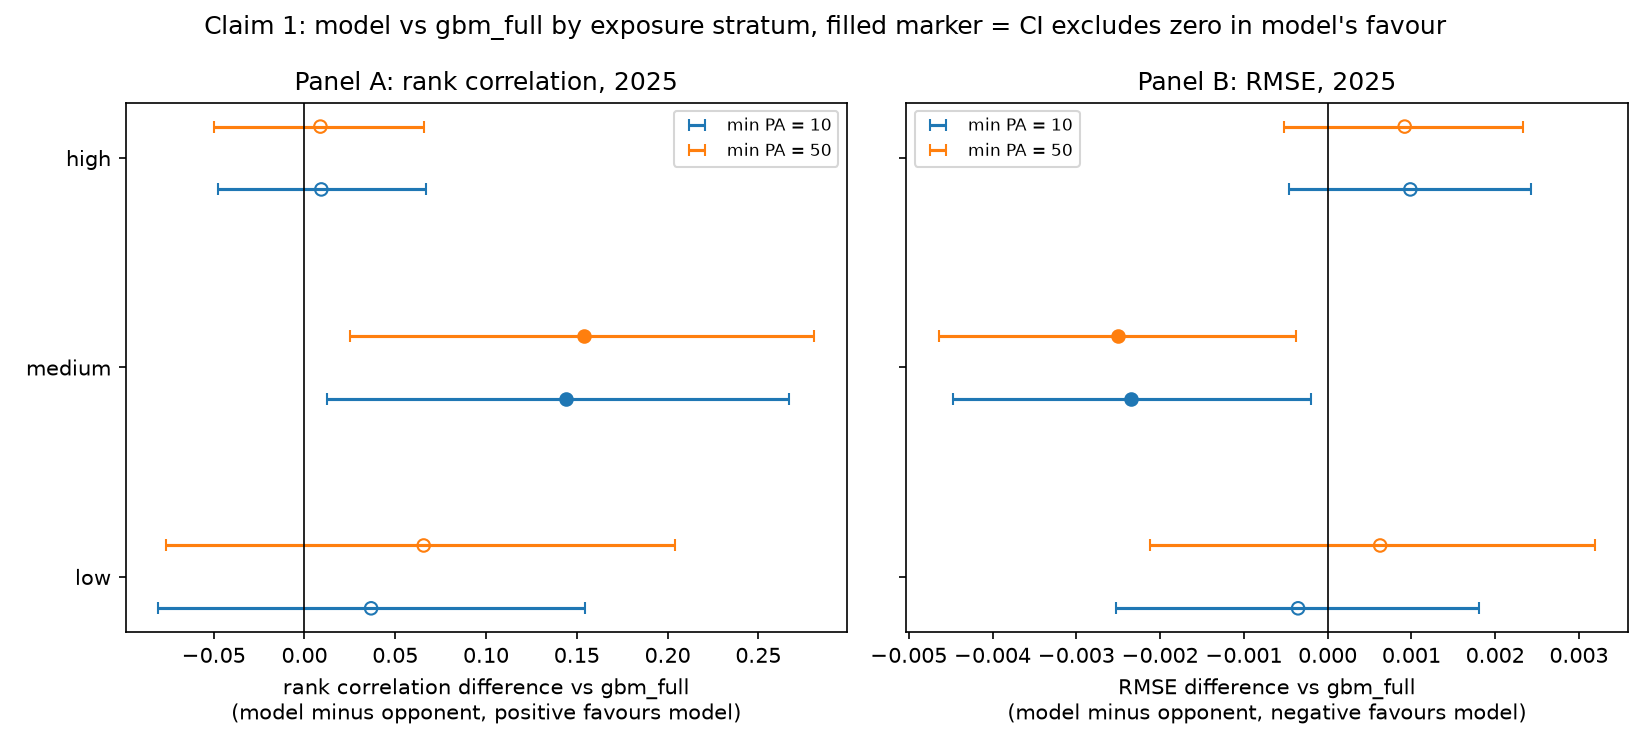
\includegraphics[width=0.85\linewidth]{fig_claim1_2025_strata.png}
\caption{\toreview 2025 results by prior-exposure stratum. The model's margin over the boosted baseline on error and order, at 10 and 50 PA evaluation floors. Only the low stratum was registered, and the medium and high strata are exploratory. The margin is largest in the medium stratum and close to zero in the high stratum.}
\label{fig:strata}
\end{figure}

% Source: results/case_studies_2025/case_studies_2025.json (all_hitters: 539, 296/243, wMAE 0.0448/0.0462,
% within_noise 519); all_hitters_bootstrap.json (2,000 batter draws, seed 0: diff -0.0014 [-0.0026, -0.0002],
% share 0.549 [0.506, 0.592]). Graded after the registered test.
Table~\ref{tab:test} scores each side of a hitter on its own. A platoon decision turns on the gap between the sides, so after the registered test we also graded each hitter's 2025 split, his wOBA against left-handers minus his wOBA against right-handers, against the model's projected split and the empirical Bayes one. This grade is exploratory. Across the 539 hitters with a 2025 split against both hands, the model's projection was closer for 296 (55\%) and empirical Bayes's for 243. Their mean absolute errors, weighted by the harmonic mean of each hitter's PA against the two hands, are 0.0448 and 0.0462. The model's error is lower by 0.0014, with an interval of 0.0002 to 0.0026 from 2,000 draws that resample hitters, and its share of closer projections has an interval of 51\% to 59\%. The edge is small next to the noise in any one hitter's split. For 519 of the 539, the observed split falls close enough to the midpoint of the two projections that noise alone could flip which one is closer.

\subsection{How much of the signal one season can measure}
\label{sec:ceiling}

% Source: results/measurement_ceiling_clean/differential_fraction_of_ceiling.csv (route B' 0.2965,
% route A 0.167); differential_exhibit.csv (achieved 0.1766, EB 0.1458, GBM 0.1413; RMSE vs floor
% 0.0633 / 0.0639; analytic fraction CI 0.264-0.910 per routes.json; 0.253-0.872 belongs to the MC 0.571); level_ceiling_level_ceiling.json
% (0.742, 0.475, 0.6406); measurement_ceiling_summary.json (coverage 0.8695). 2024, n = 545.
The 2025 margins are a few thousandths of wOBA in error and a few hundredths in pooled rank correlation, so a team's decision turns on gaps that small. That raises the question of how much of either one season of outcomes can measure at all. Even a model that knew every hitter's true talent would not match one season of outcomes, because one season of outcomes is itself noisy. Comparing the spread of hitters' observed wOBA with the spread that sampling noise alone would produce gives the share of the spread that is real, and from that share the best correlation any method could reach. For the split we estimate the spread of true splits from earlier seasons (our main estimate) and from 2024 alone (the alternative). We call that the ceiling. We compute it on 2024 with the model trained through 2023, among the 545 hitters with at least 10 PA against each hand. Because 2024 is the season we chose the model on, these numbers describe the model and are not a test of it.

For the level of a hitter's wOBA, pooled over both hands, the ceiling on rank correlation is 0.742. The model reaches 0.475, or 64\% of it. The platoon split, a hitter's wOBA against left-handers minus his wOBA against right-handers, is much harder. True splits vary little from hitter to hitter compared with the noise in a season of them, so even a perfect model would reach a rank correlation of only about 0.30 with the observed split. After removing each batting side's average split, the model reaches 0.177, 60\% of the ceiling, against 49\% for empirical Bayes and 48\% for the boosted baseline. The interval on the model's share runs from about 26\% to 91\%. The ceiling also depends on how the variance of true splits is estimated. Our main estimate, fixed as primary before it was computed, gives 0.296, and the alternative we report alongside it gives 0.167, which the model already exceeds, and that alternative falls apart if the noise estimate moves by 3\%. At this sample size no single ceiling is firm, and the 60\% should be read as a rough share. Figure~\ref{fig:ceiling} shows both ceilings.

% Source: paper/draft2/make_figs.py ceiling() from differential_exhibit.csv (pooled) and level_ceiling_level_ceiling.json.
\begin{figure}[t]
\centering
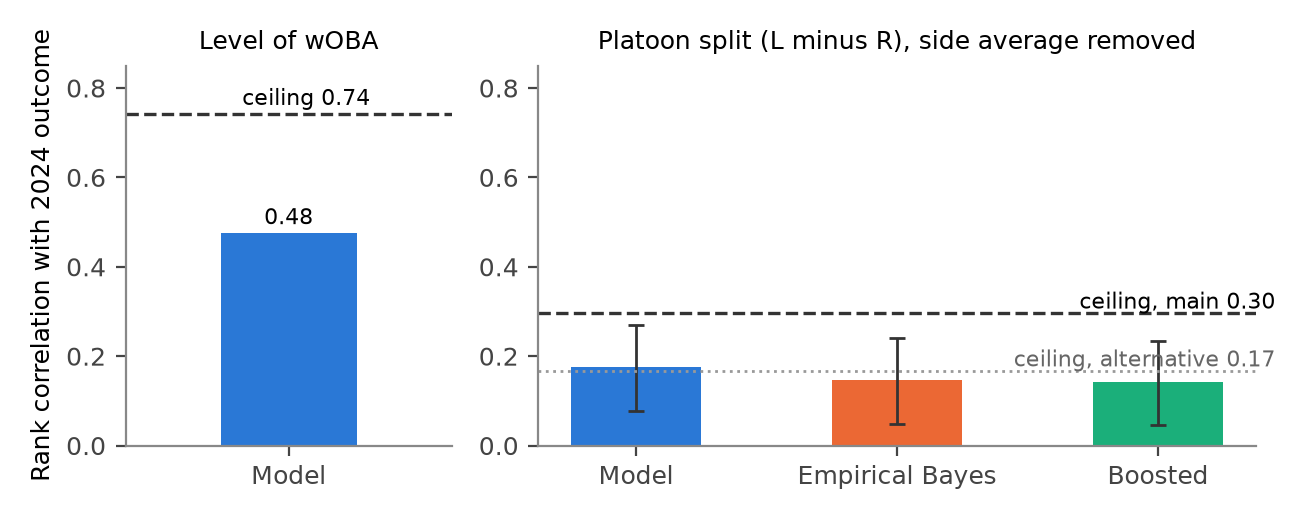
\includegraphics[width=\linewidth]{fig_ceiling.png}
\caption{\toreview Rank correlation with 2024 outcomes against the ceiling one season allows, among the 545 hitters with at least 10 PA against each hand. The left panel is the level of wOBA pooled over both hands. The right panel is the platoon split after removing each batting side's average split, with 95\% intervals from resampling hitters, the main ceiling (dashed), and the alternative ceiling (dotted). 2024 is the selection season, so the figure describes the model and tests nothing.}
\label{fig:ceiling}
\end{figure}

On error the picture is flatter. Sampling noise alone puts the floor for a platoon split's error at 0.0639, and the model's error is 0.0633, the same as the floor to within a percent. Empirical Bayes sits about as close, and the boosted baseline is slightly but measurably further from it. One season cannot say much about how many points a hitter's split is worth, for any method. That is the first sign of a pattern Section~\ref{sec:discussion} returns to, that the model is more useful for ordering hitters than for sizing their splits.

\subsection{What the embedding learned}
\label{sec:embedding}

% Source: results/v_chain_clean/embedding_structure/embedding_structure.json (norm r 0.934, PC1 r 0.090,
% silhouette max 0.054, neighbour_purity); embedding_alt_views.json (LDA 5-fold, n 1,493, power 0.791,
% contact 0.754, zone swing 0.746, chase 0.734); seed_stability_corrected_null.json (0.837 vs 0.123).
% Selection model (trained through 2023).
The embedding is trained only to predict what a hitter does with each pitch. The loss scores single pitches and never sees a hitter-level statistic such as a contact rate or a 90th-percentile exit velocity, so any such summary that shows up in the embedding was assembled by the model. We read the embedding of the selection model. A hitter's raw vector grows longer the more he has played (correlation 0.93 with log prior PA), so we scale every vector to unit length first, after which the main direction of variation has almost nothing to do with playing time (0.09). Five seeds trained from different starting points give similar vectors for the same hitter. After rotating each seed onto the first, the median cosine similarity is 0.84, against 0.12 when hitters are shuffled before the rotation is fit.

We split 1,493 hitters into thirds on attributes measured from their own pitches, then ask a linear classifier on the embedding to recover each hitter's third under five-fold cross-validation. It recovers power, measured as 90th-percentile exit velocity, for 79\% of hitters, and contact rate on swings for 75\%, against 33\% by chance. In-zone swing rate (75\%) and chase rate (73\%) come out about as well. The attributes are measured on the pitches the model trained on, so this shows what the embedding holds, not a prediction. Figure~\ref{fig:powercontact}, in the introduction, places each hitter on the fitted power and contact directions. The left panel colors hitters by their observed power third, and the right panel shows mean observed wOBA in each cell, which rises toward high power and high contact.

The same structure shows up locally. A hitter's ten nearest neighbours in the embedding share his power third 57\% of the time, against 33\% when the labels are shuffled, and 59\% against 40\% among high-exposure hitters. The embedding does not split into types, though. The silhouette score, which runs from $-1$ to 1 and is near zero when groups overlap, is at most 0.054 for any number of groups from two to ten. We therefore describe neighbourhoods and make no claim about hitter archetypes. Embedding neighbours are also not the hitters closest on results. For the five hitters in Section~\ref{sec:anchors}, lists of eight high-exposure neighbours drawn from the embedding and from observed rate statistics share 9 of 40 names.

% Source: embedding_structure/neighbour_purity.csv (stand, all, 0.682 vs null 0.506; clean build.
% Outline v4's 0.645 is the 2026-09-09 pre-clean figure); paper_figures/platoon_sign_agreement.json
% (310/545 = 0.569, null 0.498, 2024); platoon/platoon_projection.json (cosine 0.142 [0.081, 0.201],
% partial r 0.074 / 0.144 / 0.133, pooled 0.074 [0.046, 0.106], n 1,496, training-season splits).
The embedding also holds a weak platoon direction. Neighbours share a batting side 68\% of the time against 51\% by chance. After removing each batting side's average split, the model's projected 2024 split has the same sign as the observed one for 310 of 545 hitters (57\%), against 50\% when hitters are shuffled, and in the medium stratum alone that agreement is not distinguishable from chance. Nudging each of the 64 dimensions in turn and measuring how much the projected left-minus-right gap moves, averaged over 40 hitters, gives one direction along which the projected split grows (Figure~\ref{fig:direction}). It points roughly the same way as a direction fit separately to decode the empirical Bayes split from the same embedding, with a cosine of 0.14 (interval 0.08 to 0.20). Projecting every trained left- or right-handed hitter with an observed split onto it and comparing with his observed split in the training seasons, after controlling for playing time, gives a correlation of 0.07 in the low stratum, 0.14 in medium, and 0.13 in high, each with an interval above zero. The high stratum clears zero only on the clean build, and it did not on the earlier one. The structure is there, and it is small, which fits Section~\ref{sec:ceiling}, where the split is the hardest thing in the data to measure.

\begin{figure}[t]
\centering
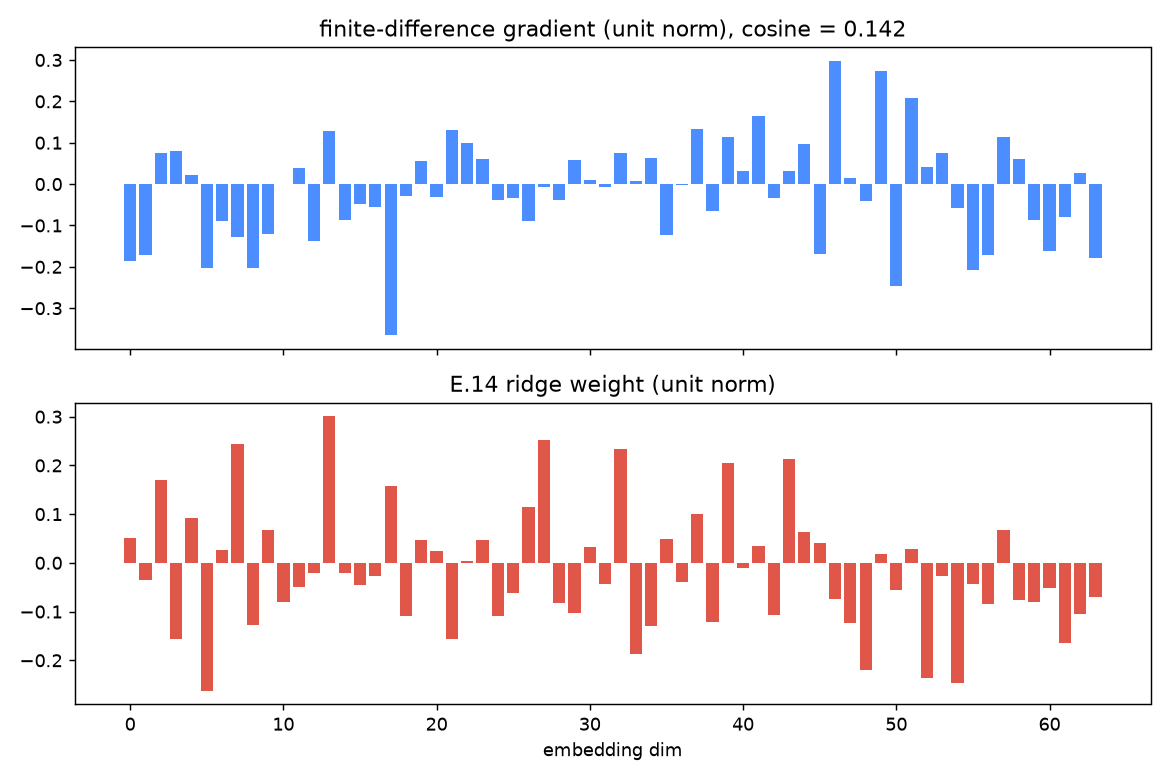
\includegraphics[width=0.85\linewidth]{fig_platoon_direction.png}
\caption{\toreview The platoon direction. The top panel is the gradient of the model's projected left-minus-right gap across the 64 embedding dimensions, and the bottom panel is the direction fit to decode the empirical Bayes split. Both are scaled to unit length.}
\label{fig:direction}
\end{figure}

% =====================================================================================
\section{Discussion}
\label{sec:discussion}

% Source: Section 3 numbers; results/case_studies_2025/case_studies_2025.{csv,json};
% results/v_chain_clean/{neighbours_high.csv, disagreement_summary.json, disagreement_top.csv,
% surfaces_summary.csv}; docs/phase-v-spec.md V.8 to V.10 (anchors and expectations, written before
% results); decision log 2026-10-31 (two entries).
\subsection{Ordering, not sizing}
\label{sec:ordering}

Our reading of these results is that the model is better at saying which of two hitters will do better against a hand than at saying by how many points. The evidence for that reading is uneven, so we give it from strongest to weakest. The strongest is the pooled 2025 ordering. The model's rank correlation beat both baselines with intervals that exclude zero while its error tied them. That comparison is exploratory, but it is out of sample. Weaker is the 2024 ceiling analysis, which is descriptive and comes from the season we chose the model on. There the model's rank correlation on the split reached 60\% of what one season allows, while its error sat at the noise floor.

Matching the noise floor is not specific to the model. Empirical Bayes sits about as close to the same floor, so on one season of outcomes no method can show much skill at sizing a split. The 2025 grade of each hitter's split points the same way. On the size of the split the model was closer slightly more often than empirical Bayes and with a slightly lower weighted error, also exploratory, so its weakness at sizing is shared with the baseline rather than its own. The model's own uncertainty is also too narrow for sizing. On 2024, its nominal 95\% prediction intervals, built from the spread of the five seeds and each unit's own sampling noise, cover the observed value 87\% of the time across all 1,149 hitter and hand units.

For a team, the order is usually what the decision needs. Choosing between two bench bats to start against a left-hander is a ranking question, and an error of a few points of wOBA in both projections does not matter if the two are in the right order. In exploratory comparisons the model's edge was largest among hitters with 113 to 451 prior PA against a hand, which is where that call is actually open. A hitter with fewer PA than that is close to unknown to every method, and a hitter with more is already well measured by the baselines. That band is a finding on one season, and we registered the band as a hypothesis for 2026 before any 2026 outcome was scored. The rule for that test is not yet fixed, and even in the medium band one season holds only about 60\% of the batters needed to detect the margin we observed with 80\% power.

\subsection{Five hitters}
\label{sec:anchors}

Before any of the analysis below was run, we picked five hitters and wrote down what the model should say about them. All five are high-exposure hitters, the stratum where no method beat the others in 2025, so they show how the model reasons about hitters it knows well rather than where its edge lies. Bohm replaced our original right-handed pick, Adam Duvall, once the training data showed Duvall had no platoon split. Joc Pederson and Kyle Schwarber are left-handed hitters with a reputation as platoon bats, so they should project worse against left-handers. Alec Bohm, a right-handed hitter, should project better against them. Mike Trout and Juan Soto are stars who play every day, so their splits should be close to flat and their neighbours should be good hitters. Table~\ref{tab:cases} gives each one's 2025 projection beside the empirical Bayes projection and what happened.

\begin{table}[t]
\centering\small
\begin{tabular}{llrrrr}
\toprule
Hitter & Bats & Model & EB & Observed (SE) & $z$ \\
\midrule
Joc Pederson & L & $-0.047$ & $-0.039$ & $+0.172$ (0.121) & 1.77 \\
Kyle Schwarber & L & $-0.042$ & $-0.028$ & $+0.025$ (0.039) & 1.52 \\
Juan Soto & L & $-0.041$ & $-0.044$ & $-0.074$ (0.041) & 0.78 \\
Mike Trout & R & $+0.009$ & $+0.007$ & $-0.062$ (0.056) & 1.25 \\
Alec Bohm & R & $+0.022$ & $+0.033$ & $+0.042$ (0.052) & 0.28 \\
\midrule
Aaron Judge & R & $+0.020$ & $+0.003$ & $+0.038$ (0.049) & 0.54 \\
José Altuve & R & $+0.021$ & $+0.026$ & $+0.013$ (0.051) & 0.22 \\
Marcell Ozuna & R & $+0.020$ & $+0.002$ & $-0.006$ (0.050) & 0.33 \\
\bottomrule
\end{tabular}
\caption{2025 platoon split (wOBA against left-handed pitchers minus wOBA against right-handed pitchers) for the five hitters chosen in advance and three of the hitters on whom the model and empirical Bayes disagreed most in 2024. SE is the standard error of the observed split, and $z$ is the distance of the observed split from the midpoint of the two projections, in standard errors. Which projection is closer depends only on which side of that midpoint the observed split falls, and every $z$ is below 1.96, so noise alone could flip each grade.}
\label{tab:cases}
\end{table}

The model's projections match four of the five expectations. Pederson and Schwarber are projected worse against left-handers, Bohm better, and Trout close to flat. Soto, expected to be flat, is projected 0.041 worse against left-handers. Inside the model, Pederson swings less than an average hitter and does more damage on balls in play against both hands, but the swing shortfall is larger, and the damage edge smaller, against left-handers. In 2025, though, empirical Bayes was closer for all five, by 0.002 to 0.014, and Figure~\ref{fig:cases} shows how far inside the noise each grade sits. Pederson shows why one season settles nothing here. Against left-handers Pederson had 19 PA in 2025 and an observed split of $+0.172$, with a standard error of 0.121, which is wide enough to hold either projection and the opposite sign as well.

Neighbours show what the model thinks a hitter is like. Restricting both lists to high-exposure hitters, Pederson's eight nearest neighbours in the embedding are Kyle Schwarber, Joey Gallo, Justin Smoak, Harrison Bader, Logan Morrison, Franmil Reyes, Ryan Zimmerman, and Matt Chapman. Four bat left-handed and four right-handed, although we had expected Pederson's neighbours to share a batting side. Two of the eight, Schwarber and Smoak, also appear among Pederson's nearest neighbours by observed rate statistics. Trout's embedding neighbours are Ronald Acuña, Pete Alonso, Brandon Belt, Eugenio Suárez, Austin Jackson, Anthony Rendon, Howie Kendrick, and Christian Walker. By rate statistics, which include wOBA itself, Trout's neighbours are Yordan Álvarez, Paul Goldschmidt, Juan Soto, Mookie Betts, Joey Votto, Rhys Hoskins, Ronald Acuña, and Will Smith. Only Acuña is on both lists. The statistics list is mostly stars. The embedding list mixes stars with ordinary regulars, and a name like Austin Jackson's is hard to defend as a peer of Trout's on results. Our reading is that the embedding compares how hitters handle pitches more than how well things turned out, and that the neighbour search compares directions and ignores the length of a hitter's vector, which is where playing time sits. The same gap shows in all five, whose two lists share only 9 of 40 names (Section~\ref{sec:embedding}).

\subsection{Where the model and empirical Bayes disagree}
\label{sec:disagree}

The model and empirical Bayes mostly agree on who has the larger platoon split. On 2024, across 545 hitters, their projected splits have a Spearman correlation of 0.77, and 0.80 and 0.79 in the low and medium strata. They disagree most among high-exposure hitters (0.69). Ranking within each batting side, the largest disagreement is Robbie Grossman, whom empirical Bayes ranks first among right-handed hitters and the model 324th. Marcell Ozuna is the reverse, 6th by the model and 316th by empirical Bayes. Aaron Judge and José Altuve are in the top ten, both ranked much higher by the model.

% Source: case_studies_2025.csv (disagreement_top rows, stratum by 2025 prior PA).
We graded these disagreements against 2025 in a separate step, so the 2024 comparison stayed descriptive as registered. Of the top twenty disagreements from 2024, 16 played in 2025, and the model was closer for 9. We start with the six of them in the medium band by 2025 prior PA, since that is the band where Section~\ref{sec:test} found the model's edge. All sixteen graded disagreements bat right-handed, so all six here do too. The model was closer for Nick Allen, Lenyn Sosa, and Jordan Walker, and empirical Bayes for Riley Adams, Luis Robert, and Chas McCormick. Robert shows how little one season settles. Both methods projected a small split, 0.004 from the model and 0.019 from empirical Bayes, and Robert's observed split was 0.091 with a standard error of 0.057, so empirical Bayes was closer only because it projected slightly more.

The three high-exposure disagreements in Table~\ref{tab:cases} show how thin each grade is. For Judge the model projected a larger split than empirical Bayes, and the observed split was larger still, so the model was closer by 0.017. For Ozuna the model made the same kind of call and the split came out near zero, so empirical Bayes was closer by 0.018. For Altuve the two projections had moved close together by 2025, and the model was closer by 0.005. Each observed split has a standard error near 0.05, about the size of the gaps being graded, and for every hitter named in this section the observed split falls close enough to the midpoint of the two projections that noise alone could flip the grade (Figure~\ref{fig:cases}). Across all 539 hitters the model was closer slightly more often (Section~\ref{sec:test}). These cases show how the model reasons, and they are not evidence that it is right.

% Source: paper/draft2/make_figs.py cases() from case_studies_2025.csv.
\begin{figure}[t]
\centering
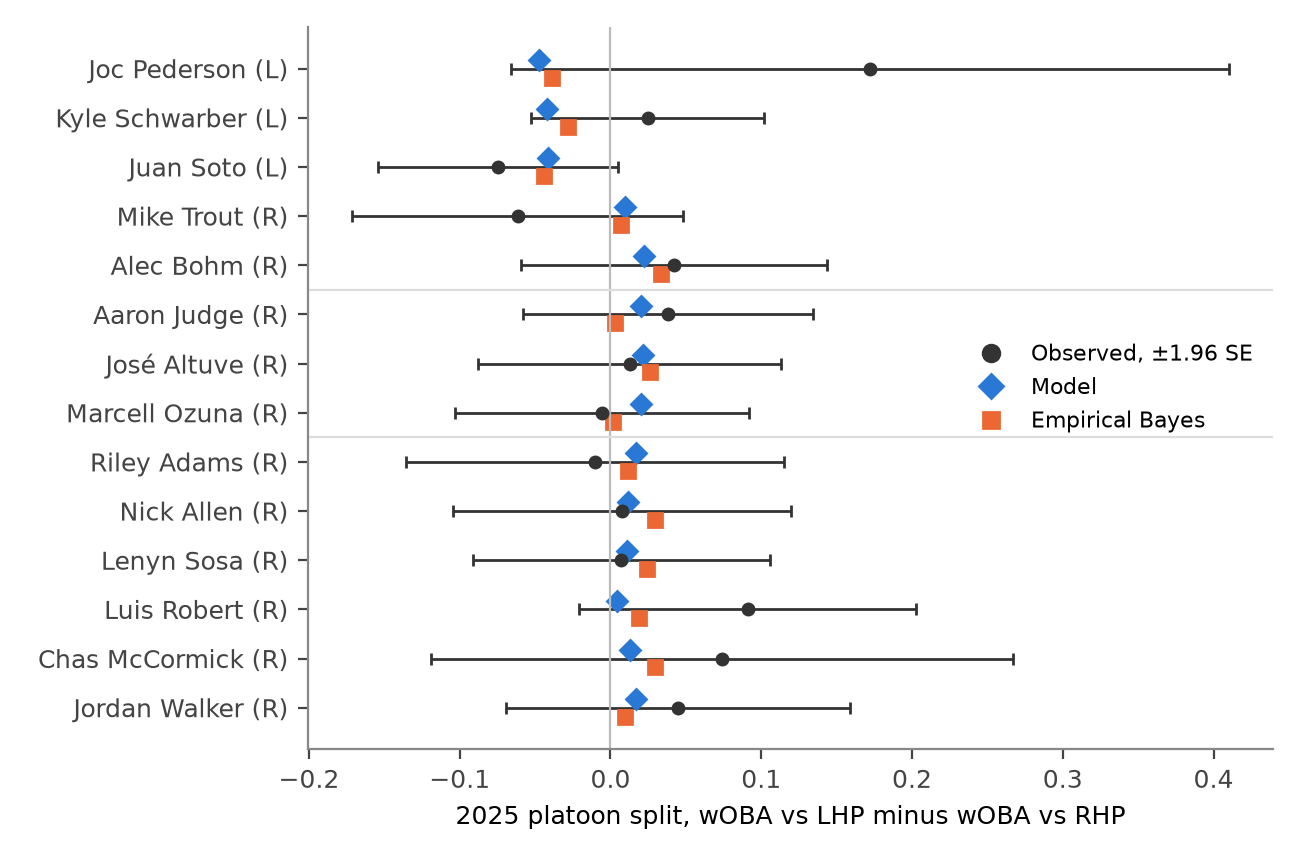
\includegraphics[width=\linewidth]{fig_cases.png}
\caption{\toreview 2025 platoon splits for the five hitters chosen in advance (top), the three high-exposure disagreements in Table~\ref{tab:cases} (middle), and the six medium-band hitters among the top twenty 2024 disagreements (bottom). Each observed split is shown with a 1.96 standard error bar beside the model's and the empirical Bayes projection. Every bar holds both projections.}
\label{fig:cases}
\end{figure}

\subsection{Limits}
\label{sec:limits}

The model did not pass the test we registered, and the result we lean on most, the medium band, is exploratory. The 2025 season was scored twice, and the second configuration was chosen by a search set up after the first score was seen (Section~\ref{sec:eval}). The ceiling is measured on the selection season and its estimate is fragile at this sample size. The model's prediction intervals are too narrow, covering 87\% of outcomes at a nominal 95\%. The count is the only game state the model sees. Cold-start hitters, 43\% of the low stratum, get one of only four projections. And any single hitter's season is noisy enough that no case study above can be read as evidence for either method.

% =====================================================================================
\section{Conclusion}
\label{sec:conclusion}

We trained a network on what hitters control on each pitch and queried it by reweighting the pitchers a projection is drawn over. On handedness splits in 2025 it tied a gradient-boosted model and empirical Bayes on error and ordered hitters better than both, and it helped most for hitters with a moderate track record against a hand. Both are exploratory results. It did not pass the test we registered.

Several things would come next. The other queries in Section~\ref{sec:query}, such as pitchers who throw hard or one named pitcher, run through the same code but have never been checked against outcomes. Each needs a held-out target and a baseline built for it. The medium band needs a fixed test rule and more data than one season, since 2026 alone holds about 60\% of the batters that test needs. The low band needs a better start for hitters the model has never seen, either a prior built from what is known about them or, as \citet{alcorn2018} suggested, minor league data mapped into the same space. The model sees only the count, and the score, inning, and runners could change what a hitter does with a pitch. Finally, the query is only useful if it reaches a decision, so the next practical step is a matchup card that ranks a team's options against a given pitcher with an honest band around each projection. That needs the model's intervals recalibrated first, since on 2024 they covered 87\% of outcomes at a nominal 95\%.

The code is at \url{https://github.com/nseluga/Hitter-Embedding}.

\clearpage
\bibliographystyle{plainnat}
\bibliography{refs}

\end{document}
